\documentclass{article}
\usepackage[T1]{fontenc}
\usepackage{lmodern}
\usepackage{graphicx}
\usepackage{amsmath,amssymb}
\usepackage[a4paper,margin=2cm]{geometry}
\usepackage[absolute,overlay]{textpos}
\setlength{\TPHorizModule}{1mm}
\setlength{\TPVertModule}{1mm}
\usepackage[indonesian]{babel}
\usepackage{hyperref}
\setlength{\emergencystretch}{2em}
% unit: Halaman 58

\begin{document}

% === Halaman 58 (llm) ===

Dekripsi

\vspace{10mm}

If you need to know about RC4 encryption algorithm, please carefully read the instructions of this tool to set relevant parameters correctly.

Input Content

5cc0adeadf45a1c2a0cb1b6527f95afa1a1cfb73d5dbd7f7173933f49139a227b088f5d06f0e35fd2cb220bb44e97b1cbeae4fa2f694dc

Password: selamat sore gaes

Charset: UTF-8

In-Format: hex

Out-Format: string

RC4 Encrypt \quad RC4 Decrypt \quad Copy \quad Clear

Output Result

Terbanglah sampai ke angkasa setinggi bintang di langit

% deskripsi: Screenshot antarmuka web alat enkripsi dan dekripsi RC4 yang menunjukkan input ciphertext hex, password 'selamat sore gaes', dan hasil dekripsi teks 'Terbanglah sampai ke angkasa setinggi bintang di langit'.
% bbox normalisasi: [0.0600, 0.1000, 0.9500, 0.9100]
\begin{textblock*}{186.90mm}(12.60mm,29.70mm)
\noindent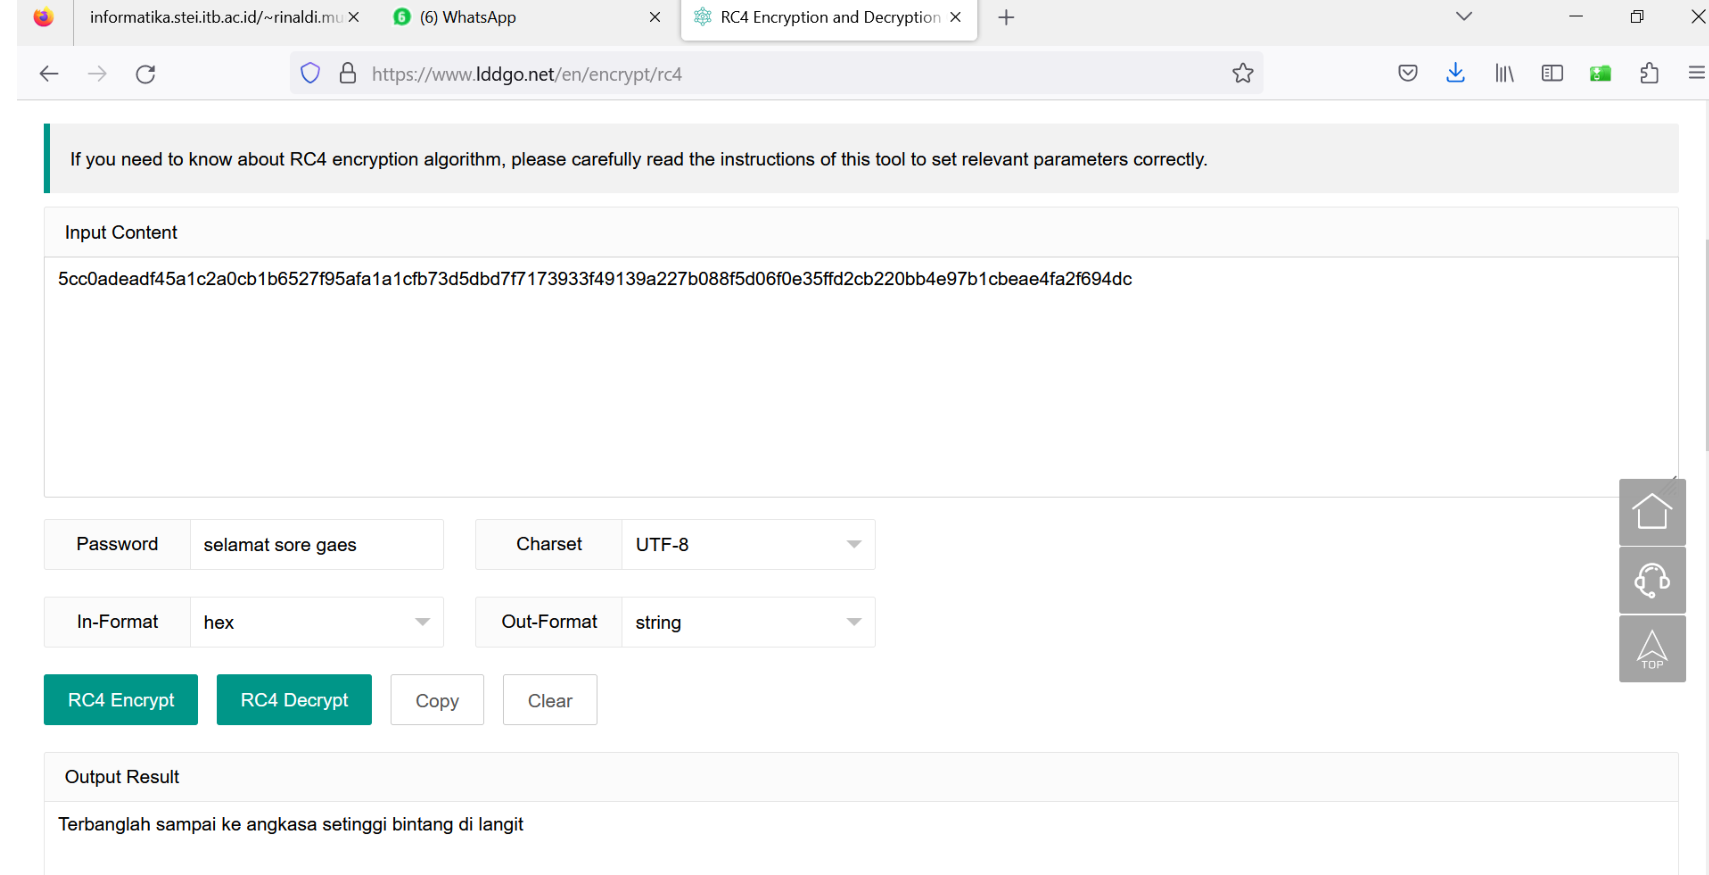
\includegraphics[width=186.90mm,height=240.57mm]{../../images/llm/page_058_img_01.png}%
\end{textblock*}

\end{document}
